\chapter{Immutable Objects}

\section{What Does Immutability Mean?}

Many people read the statement that ``Java \java{String}s are immutable'', and then write code like this:

\begin{code}
String metal;
metal = "lead";
metal = "gold";
\end{code}

and ask ``Didn't that just change the string?''  No, that code does not change lead into gold.

Let's take a look at a memory diagram after the first assignment. \java{metal} is a {\em reference} to an area of memory (called the {\bf heap}) where the string \java{"lead"} has been allocated.

\begin{figure}[!h]
\begin{center}
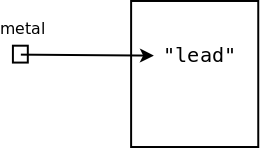
\includegraphics[scale=0.4]{figs/ch09/heap1.png}
\caption{Reference to a String on the heap}
\label{fig.heap1}
\end{center}
\end{figure}

After the second assignment, the {\em reference} has changed to refer to another portion of the heap that contains the string \java{"gold"}. The string \java{"lead"} is still on the heap, unmodified. It's just that nobody is referring to it any longer.

\begin{figure}[!h]
\begin{center}
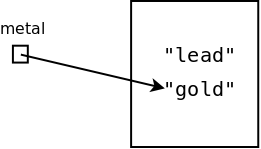
\includegraphics[scale=0.4]{figs/ch09/heap2.png}
\caption{Reference to a second String on the heap}
\label{fig.heap2}
\end{center}
\end{figure}

What would ``changing the string'' look like? In some languages, a string is treated as if it were an array of characters, and you could write code like this:

\begin{code}
metal = "gold";
metal[0] = 's'; // change first letter to 's'
\end{code}

Java won't let you do that because the string itself, which is out there on the heap, cannot be modified.

\begin{figure}[!h]
\begin{center}
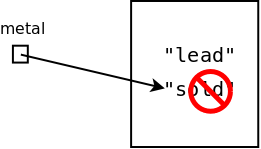
\includegraphics[scale=0.4]{figs/ch09/bad_heap.png}
\caption{Non-Java modified string (illegal in Java)}
\label{fig.bad.heap}
\end{center}
\end{figure}

But there's nothing to stop you from creating a brand new \java{String} on the heap and changing the value of \java{metal} to refer to that new \java{String}, as shown in Figure~\ref{fig.heap3}:

\begin{code}
metal = "s" + metal.substring(1, 4);
\end{code}

\begin{figure}[!h]
\begin{center}
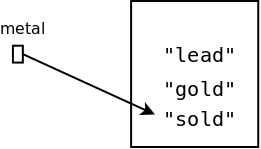
\includegraphics[scale=0.4]{figs/ch09/heap3.png}
\caption{Reference to a newly created String on the heap}
\label{fig.heap3}
\end{center}
\end{figure}

\clearpage

\section{Generalizing and the \java{Scanner} Class}

The {\em Think Java} book's subtitle is ``How to Think Like a Computer Scientist,'' and in that spirit, places more emphasis on the concepts of computer science---developing and analyzing algorithms. In order to do this, the book deliberately avoids going into the minutiae of the Java language. At this point, however, we have to get into a detail of the \java{Scanner} class that comes up when you are generalizing and modularizing your code.

Whenever you generalize a method for doing input, do {\em not} create the \java{Scanner} inside the method. Instead, you must pass a \java{Scanner} object as one of the parameters.

Consider the following program that asks a user for two prices and calculates the percentage change:

\begin{code}
import java.util.Scanner;

public class RepeatedCode {
  public static void main(String[] args) {
    Scanner input = new Scanner(System.in);
    double originalPrice;
    do {
      System.out.print("Enter original price: ");
      originalPrice = input.nextDouble();
      if (originalPrice <= 0) {
        System.out.println("Price must be greater than zero.");
      }
    } while (originalPrice <= 0);
    
    double newPrice;
    do {
      System.out.print("Enter new price: ");
      newPrice = input.nextDouble();
      if (newPrice <= 0) {
        System.out.println("Price must be greater than zero.");
      }
    } while (newPrice <= 0);
    
    double pctChange = 100.0 *
      (newPrice - originalPrice) / originalPrice;
    System.out.printf("Price change: %.1f%%\n", pctChange);
  }
}
\end{code}

The code for the two inputs is identical except for the prompt (and the variable name). Here is a way to generalize that code by creating a method to get the input and having the input prompt as its parameter:

\begin{code}
import java.util.Scanner;

public class GeneralInput1 {
  
  public static double getPrice(String prompt) {
    Scanner input = new Scanner(System.in);
    double price;
    do {
      System.out.print(prompt);
      price = input.nextDouble();
      if (price <= 0) {
        System.out.println("Price must be greater than zero.");
      }
    } while (price <= 0);
    return price;
  }

    
  public static void main(String[] args) {
    double originalPrice = getPrice("Enter original price: ");
    double newPrice = getPrice("Enter new price: ");
    double pctChange = 100.0 *
      (newPrice - originalPrice) / originalPrice;
    System.out.printf("Price change: %.1f%%\n", pctChange);
  }
}
\end{code}

This program works, but there's a trap hidden in it. Every time the code calls \java{getPrice}, a new \java{Scanner} is created, opening a new connection to the keyboard. This is inefficient, but not fatal---until someone tells you that you should always close an I/O device and you add the code \java{input.close();} between the end of the loop and the \java{return} statement.

Once the \java{input} is closed, its connection to the keyboard is broken {\em and cannot be re-opened}. Now, when you run the program, you get this result:

\begin{stdout}
Enter original price: 3.50
Enter new price: Exception in thread "main"
  java.util.NoSuchElementException
        at java.base/java.util.Scanner.throwFor(Scanner.java:937)
        at java.base/java.util.Scanner.next(Scanner.java:1594)
        at java.base/java.util.Scanner.nextDouble(Scanner.java:2564)
        at BadClose.getPrice(BadClose.java:10)
        at BadClose.main(BadClose.java:22)
\end{stdout}

In order to avoid the minor problem of creating multiple connections to the keyboard and the major problem of inadvertently closing the connection before you want to, your code must create the \java{Scanner} once, and once only. Here is code that solves the problem. It creates the \java{Scanner} once in \java{main}, closes it only once the end of \java{main}, and passes it as an additional argument to the \java{getPrice} method:

\begin{code}
import java.util.Scanner;

public class GeneralInput2 {
  
  public static double getPrice(Scanner in, String prompt) {
    double price;
    do {
      System.out.print(prompt);
      price = in.nextDouble();
      if (price <= 0) {
        System.out.println("Price must be greater than zero.");
      }
    } while (price <= 0);
    return price;
  }

    
  public static void main(String[] args) {
    Scanner input = new Scanner(System.in);
    double originalPrice = getPrice(input, "Enter original price: ");
    double newPrice = getPrice(input, "Enter new price: ");
    double pctChange = 100.0 *
      (newPrice - originalPrice) / originalPrice;
    System.out.printf("Price change: %.1f%%\n", pctChange);
    input.close();
  }
}
\end{code}

\section{Exercises}

\begin{exercise}
In this exercise, we will once again rewrite the ``dew point'' program. Prompt the user for the air temperature in degrees Celsius and the relative humidity as a percent, and calculate the dew point with this formula:

\begin{equation*}
dewPoint = temperature - {{100 - relHumidity} \over 5}
\end{equation*}

Generalize the code to use a method to get the temperature. This method should accept only numbers in the range -90 to 60 degrees Celsius, giving an error message if the temperature is out of range. (The range given here includes the lowest and highest recorded temperatures on earth.)

Write a method to get the relative humidity. This method should accept only numbers in the range 0 to 100, giving an error message if the relative humidity is out of range.

Here is what output might look like when the user enters several out-of-range values:

\begin{stdout}
Enter temperature in degrees C: 85
Value must be in range -90 to 60.
Enter temperature in degrees C: -100
Value must be in range -90 to 60.
Enter temperature in degrees C: 20
Enter relative humidity as a percent: -20
Value must be in range 0 to 100.
Enter relative humidity as a percent: 105
Value must be in range 0 to 100.
Enter relative humidity as a percent: 80
The dew point is 16.0 degrees C.
\end{stdout}

Can you generalize further to use only one method to get both values?  Hint: That method would need a \java{Scanner}, a prompt string, a minimum, and a maximum value as its parameters.
\end{exercise}

\begin{exercise}
There are two ways to represent latitudes and longitudes. One is as a decimal degree: 35.47°, and the other is as degrees, minutes, and seconds: 35° 28$^\prime$ 12$^{\prime\prime}$ (also called ``DMS'' format).

Write a command-line program named {\em Angle.java} that converts between these formats. The program will get its input from command line arguments.

\begin{itemize}
\item If there is only one argument, it is presumed to be an angle in decimal format, and your program will convert it to degree-minute-second format.
\item If there are two arguments, they are presumed to be degrees and minutes, and your program will convert it to decimal format.
\item If there are three arguments, they are presumed to be degrees, minutes, and seconds; and your program will convert it to decimal format.
\item For any other number of arguments, print a usage message.
\end{itemize}

Here is an example of running the program several times:

\begin{stdout}
> java Angle
Usage: Angle decimaldegrees|deg min sec
> java Angle 37.272
37° 16′ 19″
> java Angle -20 16
-20.267°
> java Angle 10 47 11
10.786°
> java Angle 66 10 47 11
Usage: Angle decimaldegrees|deg min sec
\end{stdout}

Hints:
\begin{itemize}
\item The degree symbol ° is \java{"\\u00b0"}; the minutes symbol ′ is \java{"\\u2032"}, and the seconds symbol ″ is \java{"\\u2033"}.
\item In order to handle negative angles correctly, you might find the \java{Math.signum} method useful. It takes a \java{double} as an argument and returns -1.0 if the argument is negative, 0.0 if the argument is zero, and 1.0 if the argument is positive.
\item Generalize by writing a \java{toDMS} method that takes a decimal degree and returns an array of three integers. Write another method named \java{toDecimal} which takes three parameters (degrees, minutes, and seconds) and returns the decimal equivalent as a \java{double}.
\end{itemize}

\end{exercise}

\begin{exercise}
Write a command-line program that accepts two numbers and a string representing an arithmetic operation: \java{"plus"}, \java{"minus"}, \java{"times"}, and \java{"div"} in either upper or lower case and evaluates the resulting expression.

Examples of running the program (source in {\em Calc.java}) several times:

\begin{stdout}
> java Calc
Usage: number plus|minus|times|div number
> java Calc 3 plus 4.5
7.5
> java Calc 7.5 div 2
3.75
> java Calc 6 MINUS 1.25
4.75
> java Calc 7 blah 5
Unknown operation blah
\end{stdout}

The reason this program uses words instead of the symbols \java{+}, \java{-}, \java{*}, and \java{/} is that some of these characters are interpreted by the MacOS, Windows, and Linux command lines as wild card characters or part of a file name.
\end{exercise}

